\documentclass{beamer}

%% \documentclass[handout]{beamer}
%% % use this with the [handout] option to create handouts for the audience
%% \usepackage{pgfpages}
%% \pgfpagesuselayout{2 on 1}[a4paper,border shrink=5mm]

\mode<presentation>
{
  \usetheme{Diku}
% set this to your preferences:
  \setbeamercovered{invisible}
%  \setbeamercovered{transparent}
}

\usepackage{graphicx}
\usepackage{epic}

\usepackage{amsmath}
\usepackage{amssymb}
\usepackage{amsthm}

\newcommand{\basetop}[1]{\vtop{\vskip-1ex\hbox{#1}}}
\newcommand{\source}[1]{\let\thefootnote\relax\footnotetext{\scriptsize\textcolor{kugray1}{Source: #1}}}

% for coloured code citation in text:
\usepackage{fancyvrb}

%%%%%%%%%%%%%%%%%%%%%%%%%%%%%%%%%
%%%%%    code sections   %%%%%%%%
%%%%%%%%%%%%%%%%%%%%%%%%%%%%%%%%%

% code highlighting commands in own block
\DefineVerbatimEnvironment{code}{Verbatim}{fontsize=\scriptsize}
\DefineVerbatimEnvironment{icode}{Verbatim}{fontsize=\scriptsize}

% Fancy code with color commands:
\DefineVerbatimEnvironment{colorcode}%
        {Verbatim}{fontsize=\scriptsize,commandchars=\\\{\}}

%%%%%%%%%%%%%%%%%%%%%%%%%%%%%%%%%%
%%%%%    some coloring    %%%%%%%%

\definecolor{Red}{RGB}{220,50,10}
\definecolor{Blue}{RGB}{0,51,102}
\definecolor{Yellow}{RGB}{102,51,0}
\definecolor{Orange}{RGB}{178,36,36}
\definecolor{Grey}{RGB}{180,180,180}
\definecolor{Green}{RGB}{20,120,20}
\definecolor{Purple}{RGB}{160,50,100}
\newcommand{\red}[1]{\textcolor{Red}{{#1}}}
\newcommand{\blue}[1]{\textcolor{Blue}{{#1}}}
\newcommand{\yellow}[1]{\textcolor{Yellow}{{#1}}}
\newcommand{\orange}[1]{\textcolor{Orange}{{#1}}}
\newcommand{\grey}[1]{\textcolor{Grey}{{#1}}}
\newcommand{\green}[1]{\textcolor{Green}{{#1}}}
\newcommand{\purple}[1]{\textcolor{Purple}{{#1}}}




% use "DIKU green" from our color theme for \emph
\renewcommand{\emph}[1]{\textcolor{structure}{#1}}
% use some not-too-bright red for an \emp command
\definecolor{DikuRed}{RGB}{130,50,32}
\newcommand{\emp}[1]{\textcolor{DikuRed}{ #1}}
\definecolor{CosGreen}{RGB}{10,100,70}
\newcommand{\emphh}[1]{\textcolor{CosGreen}{ #1}}
\definecolor{CosBlue}{RGB}{55,111,122}
\newcommand{\emphb}[1]{\textcolor{CosBlue}{ #1}}
\definecolor{CosRed}{RGB}{253,1,1}
\newcommand{\empr}[1]{\textcolor{CosRed}{ #1}}

\newcommand{\mymath}[1]{$ #1 $}
\newcommand{\myindx}[1]{_{#1}}
\newcommand{\myindu}[1]{^{#1}}

\newcommand{\Fasto}{\textsc{Fasto}\xspace}


%%%%%%%%%%%%%%%%%%%%

\title[Loop Parallelism]{Loop Parallelism I}

\author[C.~Oancea]{Cosmin E. Oancea\\{\tt cosmin.oancea@diku.dk}}

\institute{Department of Computer Science (DIKU)\\University of Copenhagen}


\date[Sept 2014]{September 2014 PMPH Lecture Notes}


\begin{document}

\titleslide

\begin{frame}
\frametitle{Course Organization}

\begin{tabular}{lccccc}
W  & HARDWARE  & & SOFTWARE     & & LAB/CUDA \\\hline\hline
1 & Trends         &                         & List HOM     & & Intro \& Simple\\
  & Vector Machine & $\longleftarrow$ & (Map-Reduce) & & Map Programming\\\hline
%
2 & In Order & $\longrightarrow$ & VLIW Instr   & & Scan \&\\
  & Processor& $\longleftarrow$ & Scheduling   & & Reduce \\\hline
%
3 & Cache     & & \emp{Loop}          & & Sparse Vect\\
  & Coherence & & \emp{Parallelism I} & & Matrix Mult\\\hline
%
4 & Interconnection & & Case Studies \&   & & Transpose \& Matrix\\
  & Networks        & & Optimizations   & & Matrix Mult\\\hline
%
5 & Memory      & & Optimising   & & Sorting \& Profiling \& \\
  & Consistency & & Locality     & & Mem Optimizations \\\hline
%
6 & OoO, Spec   & & Thread-Level   & & Project \\
  & Processor   & & Speculation    & & Work    \\\hline

%\framebox{Processor}       & & \framebox{Low-Level\\Optimizations}        & & \framebox{CUDA: Scan\\Reduce}\\
%$\downarrow$ && $\uparrow$ \\
%\framebox{\red Intermediate code generation} &$\longrightarrow$ & Intermediate code
\end{tabular}
\medskip
%\alert{Keywords: Reasoning, Tradeoffs, Common Case, }

Three narative threads: the path to complex \& good design: 
\begin{itemize}
    \item \emp{Design Space} tradeoffs, constraints, common case, trends.
    \item \emp{Reasoning}: from simple to complex, \emp{Applying Concepts}.
\end  {itemize}
\end{frame}



%%%%%%%% real content starts here %%%%%%%%%%

\begin{frame}
  \frametitle{Motivation}

\begin{itemize}
    \item[+] So far we reasoned about how to parallelize a known algorithm
    \item[+] using a clean, functional approach, e.g., flattening, 
    \item[+] which provides work and depth guarantees,
    \item[\alert{-}] but does \alert{NOT} account for locality of reference.

\end  {itemize}\bigskip

\emp{Why do we have to look at imperative loops?}
\begin{itemize}    
    \item A lot of legacy sequential imperative code, C{\tt++}/Java/Fortran.\medskip
    \item Need to parallelize the implementation of unknown algorithm,\medskip
    \item Need to optimize parallelism, e.g., locality of reference requires subscript analysis. 
\end  {itemize}  

\end{frame}


\section{Direction-Vector Analysis}

\begin{frame}[fragile]
	\tableofcontents[currentsection]
\end{frame}


\begin{frame}[fragile,t]
  \frametitle{Problem Statement} % of CPU, Multicores, GPGPU

%[fontsize=\small]
\begin{block}{Three Loop Examples}
\begin{colorcode}
DO i = 1, N             DO i = 2, N                 DO i = 2, N
  DO j = 1, N             DO j = 2, N                 DO j = 1, N 
    A[j,i] = A[j,i] ..      A[j,i] = A[j-1,i-1]...        A[i,j] = A[i-1,j+1]...
  ENDDO                     B[j,i] = B[j-1,i]...      ENDDO
ENDDO                   ENDDO ENDDO                 ENDDO
\end{colorcode}
\end{block} 

Iterations are ordered {\em lexicographically}, i.e., in the order
they occur in the sequential execution, e.g., 
{\tt$\vec{k}=$(i=2,j=4) < $\vec{l}=$(i=3,j=3)}.

\bigskip

\begin{itemize}
    \item \emp{Which of the three loop nests is amenable to parallelization?}\smallskip
    \item Loop interchange is one of the most simple and useful code transformations,
            e.g., used to enhance locality of reference, parallel-loop granularity,
            and even to ``create'' parallelism.\smallskip
    \item \emp{In which loop nest is it safe to interchange the loops?}
\end{itemize}


\end{frame}

\begin{frame}[fragile,t]
  \frametitle{Definition of a Dependency} % of CPU, Multicores, GPGPU

\begin{block}{Load-Store Classification of Dependencies}
\begin{colorcode}
True Dependency (RAW)    Anti Dependency (WAR)    Output dependency (WAW)
S1    X  = ..            S1    .. = X             S1    X = ...            
S2    .. = X             S2    X  = ..            S2    X = ...
\end{colorcode}
\end{block} 

\smallskip

{\bf Th. Loop Dependence:} There is a dependence from statement $S1$ to $S2$
in a loop nest {\em iff} $\exists$ iterations $\vec{k}$, $\vec{l}$ such that:
\begin{description}
    \item[1.] $\vec{k} < \vec{l}$ or $\vec{k} = \vec{l}$ and $\exists$ 
                an execution path from statement $S1$ to statement $S2$ \emp{such that:}
    \item[2.] $S1$ accesses memory location $M$ on iteration $\vec{k}$, and
    \item[3.] $S2$ accesses memory location $M$ on iteration $\vec{l}$, and
    \item[4.] one of these accesses is a write.
\end{description}
\medskip

\emp{We say that $S1$ is the source and $S2$ is the sink of the dependence}, 
because $S1$ executes before $S2$ in the sequential program execution.

\medskip
We are most interested in cross iteration dependencies, i.e., $\vec{k} < \vec{l}$.\\\smallskip
Intra iteration dependencies, i.e., $\vec{k} = \vec{l}$ are analysed for ILP. 

\end{frame}


\begin{frame}[fragile,t]
  \frametitle{Loop-Nest Dependencies} % of CPU, Multicores, GPGPU

{\em Lexicographic ordering}, 
e.g., {\tt$\vec{k}=$(i=2,j=4) < $\vec{l}=$(i=3,j=3)}.

%[fontsize=\small]
\begin{block}{Three Loop Examples}
\begin{colorcode}
DO i = 1, N             DO i = 2, N                 DO i = 2, N
  DO j = 1, N             DO j = 2, N                 DO j = 1, N 
    A[j,i] = A[j,i] ..      A[j,i] = A[j-1,i-1]...        A[i,j] = A[i-1,j+1]...
  ENDDO                     B[j,i] = B[j-1,i]...      ENDDO
ENDDO                   ENDDO ENDDO                 ENDDO
\end{colorcode}
\end{block} 
\pause

\hspace{-3ex}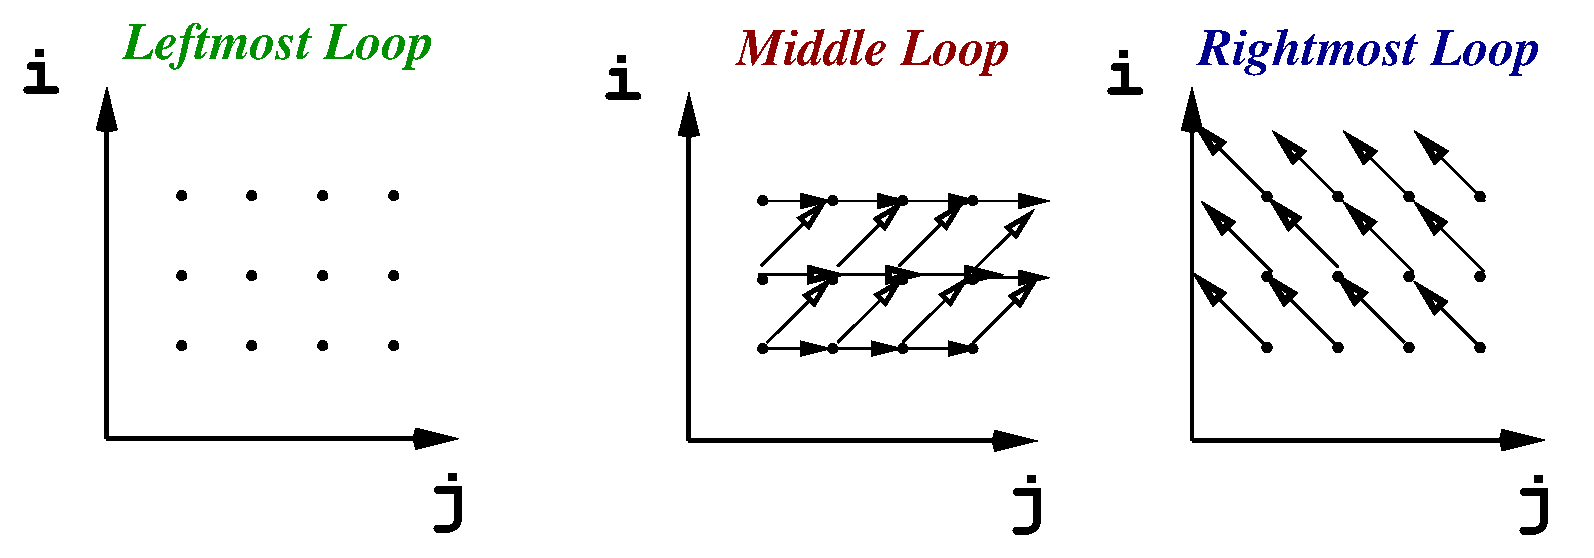
\includegraphics[height=23ex]{ParTeaserFigs/LoopDeps}  

\alert{How can I summarize this information?} %Do I have to consider all cases?

\end{frame}





\begin{frame}[fragile,t]
  \frametitle{Aggregate Dependencies via Direction Vectors} % of CPU, Multicores, GPGPU

\begin{block}{Write the Direction Vectors for Each Loop:}
\begin{colorcode}
  DO i = 1, N            DO i = 2, N               DO i = 2, N
    DO j = 1, N            DO j = 2, N               DO j = 1, N 
S1    A[j,i]=A[j,i]..  S1   A[j,i]=A[j-1,i]...   S1    A[i,j]=A[i-1,j+1]...
    ENDDO              S2   B[j,i]=B[j-1,i-1]...     ENDDO
  ENDDO                  ENDDO ENDDO               ENDDO
\end{colorcode}
\end{block} 



\smallskip

Dependencies depicted via an edge {\em from} the stmt that executes first
in the loop nest, i.e., {\em the source}, {\em to} the one that executes later, {\em the sink}.

\smallskip

{\bf Def. Dependence Direction:} Assume $\exists$ a dependence from $S1$ in iteration $\vec{k}$
to $S2$ in $\vec{l}$ ($\vec{k}\leq\vec{l}$). 
\emp{\em Dependence-direction vector $\vec{D}(\vec{k},\vec{l})$}:
\begin{description}
    \item[1.] $\vec{D}(\vec{k},\vec{l})_m = $~``{\tt{}<}'' if $\vec{k}_m < \vec{l}_m$,
    \item[2.] $\vec{D}(\vec{k},\vec{l})_m = $~``{\tt{}=}'' if $\vec{k}_m = \vec{l}_m$,
    \item[3.] $\vec{D}(\vec{k},\vec{l})_m = $~``{\tt{}>}'' if $\vec{k}_m > \vec{l}_m$.
\end{description}

\medskip
If the source is a write and the sink a read then {\sc raw} dependency,\\iIf the source is a read then {\sc war}, if both are writes then {\sc waw}.  
\end{frame}


\begin{frame}[fragile,t]
  \frametitle{Parallelism and Loop Interchange} % of CPU, Multicores, GPGPU

\begin{block}{Direction Vectors/Matrix for Three Loops }
\begin{columns}
\column{0.27\textwidth}
\begin{colorcode}
  DO i = 1, N
    DO j = 1, N
S1    A[j,i]=A[j,i]..
    ENDDO
  ENDDO
For S1\mymath{\rightarrow}S1: 
    (j1,i1)=(j2,i2) 
    i1 \emp{=} i2 \& j1 \emp{=} j2

Direction matrix:
S1\mymath{\rightarrow}S1: \emp{[=,=]}
\end{colorcode}
\column{0.32\textwidth}
\begin{colorcode}
  DO i = 2, N
    DO j = 2, N
S1    A[j,i]=A[j-1,i]...
S2    B[j,i]=B[j-1,i-1]...
    ENDDO
  ENDDO
S1\mymath{\rightarrow}S1: (j1,i1)=(j2-1,i2)
        i1 \emp{=} i2 \& j1 \emp{<} j2
S2\mymath{\rightarrow}S2: (j1,i1)=(j2-1,i2-1)
        i1 \emp{<} i2 \& j1 \emp{<} j2
S1\mymath{\rightarrow}S1: \emp{[=,<]}
S2\mymath{\rightarrow}S2: \emp{[<,<]}
\end{colorcode}
\column{0.32\textwidth}
\begin{colorcode}
  DO i = 2, N
    DO j = 1, N
S1    A[i,j]=A[i-1,j+1]...
    ENDDO
  ENDDO
For S1\mymath{\rightarrow}S1: 
    (i1,j1) = (i1-1,j2+1)
    i1 \emp{<} i2 \& j1 \emp{>} j2

Direction matrix:
S1\mymath{\rightarrow}S1: \emp{[<,>]}
\end{colorcode}
\end{columns}
\end{block} 

{\bf Th. Parallelism:} A loop in a loop nest is parallel {\em iff} all its directions
are either {\tt =} or there exists an outer loop whose corresp. direction is {\tt <}. 

\smallskip

\alert{A direction vector cannot have $>$ as the first non-= symbol},\\
as that would mean that I depend on something in the future. 
\end{frame}

\begin{frame}[fragile,t]
  \frametitle{Parallelism and Loop Interchange} % of CPU, Multicores, GPGPU

\begin{block}{Direction Vectors/Matrix for Three Loops }
\begin{columns}
\column{0.27\textwidth}
\begin{colorcode}
  DO i = 1, N
    DO j = 1, N
S1    A[j,i]=A[j,i]..
    ENDDO
  ENDDO
For S1\mymath{\rightarrow}S1: 
    (j1,i1)=(j2,i2) 
    i1 \emp{=} i2 \& j1 \emp{=} j2

Direction matrix:
S1\mymath{\rightarrow}S1: \emp{[=,=]}
\end{colorcode}
\column{0.32\textwidth}
\begin{colorcode}
  DO i = 2, N
    DO j = 2, N
S1    A[j,i]=A[j-1,i]...
S2    B[j,i]=B[j-1,i-1]...
    ENDDO
  ENDDO
S1\mymath{\rightarrow}S1: (j1,i1)=(j2-1,i2)
        i1 \emp{=} i2 \& j1 \emp{<} j2
S2\mymath{\rightarrow}S2: (j1,i1)=(j2-1,i2-1)
        i1 \emp{<} i2 \& j1 \emp{<} j2
S1\mymath{\rightarrow}S1: \emp{[=,<]}
S2\mymath{\rightarrow}S2: \emp{[<,<]}
\end{colorcode}
\column{0.32\textwidth}
\begin{colorcode}
  DO i = 2, N
    DO j = 1, N
S1    A[i,j]=A[i-1,j+1]...
    ENDDO
  ENDDO
For S1\mymath{\rightarrow}S1: 
    (i1,j1) = (i1-1,j2+1)
    i1 \emp{<} i2 \& j1 \emp{>} j2

Direction matrix:
S1\mymath{\rightarrow}S1: \emp{[<,>]}
\end{colorcode}
\end{columns}
\end{block} 

{\bf Th. Loop Interchange:} A column permutation of the loops in a loop nest 
is legal {\em iff} permuting the direction matrix in the same way {\em does NOT result}
in a {\tt >} direction as the leftmost non-{\tt{}=} direction in a row. 

\end{frame}


\begin{frame}[fragile,t]
  \frametitle{Parallelism and Loop Interchange} 

\begin{block}{Direction Vectors/Matrix for Three Loops }
\begin{colorcode}
  DO i = 1, N            DO i = 2, N               DO i = 2, N
    DO j = 1, N            DO j = 2, N               DO j = 1, N 
S1    A[j,i]=A[j,i]..  S1   A[j,i]=A[j-1,i]...   S1    A[i,j]=A[i-1,j+1]...
    ENDDO              S2   B[j,i]=B[j-1,i-1]...     ENDDO
  ENDDO                  ENDDO ENDDO               ENDDO

For S1\mymath{\rightarrow}S1: j1 = j2    For S1\mymath{\rightarrow}S1: j1 = j2-1          For S1\mymath{\rightarrow}S1: i1 = i2-1
            i1 = i2                i1 = i2                    j1 = j2+1
(i2,j2)-(i1,j1)=         (i2,j2)-(i1,j1)=\emp{[=,<]}        (i2,j2)-(i1,j1)=\emp{[<,>]}
\emp{[=,=]}                  For S2\mymath{\rightarrow}S2: j1 = j2-1
                                   i1 = i2-1
                         (i2,j2)-(i1,j1)=\emp{[<,<]}
\end{colorcode}
\end{block} 

Interchange is safe for the first and second nests, but not for the third!\\
e.g., \emp{\tt [=,<]}$~~~\rightarrow~~~$ \emph{\tt [<,=]}$~~~~~~~~~$(for the second loop nest)\\
$~~~~~~$\emp{\tt [<,<]}$~~~~~~~~~~~~$\emph{\tt [<,<]}

\pause\smallskip

After interchange, loop $j$ of the second loop nest is parallel.

\bigskip

\emph{\bf Corollary: A parallel loop can be always interchanged inwards.}
\end{frame}


\begin{frame}[fragile,t]
  \frametitle{Dependency Graph and Loop Distribution} 

{\bf Def. Dependency Graph:} edges from the source of the dependency, i.e., early iteration, 
to the sink, i.e., later iteration. 

\smallskip

{\bf Th. Loop Distribution:} Statements that are in a dependence cycle remain in one 
(sequential) loop.   The others are distributed to separate loops in graph order; 
if no cycle then parallel loops.\smallskip

\begin{block}{Vectorization Example: Remember Vector Machines?}
\begin{columns}
\column{0.34\textwidth}
\begin{colorcode}[fontsize=\scriptsize]
  DO i = 3, N
\emp{S1  A[i] = B[i-2] ...}
\alert{S2  B[i] = B[i-1] ...}
  ENDDO  

For S2\mymath{\rightarrow}S1: i1 = i2-2, \emp{[<]}
For S2\mymath{\rightarrow}S2: i1 = i2-1, \emp{[<]}
\end{colorcode}
\column{0.27\textwidth}\pause
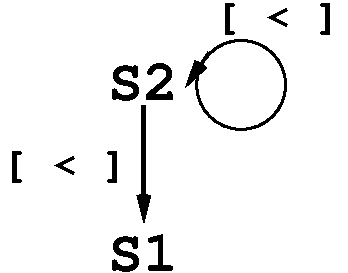
\includegraphics[height=12ex]{ParTeaserFigs/LoopDistr}  
\column{0.30\textwidth}
\begin{colorcode}[fontsize=\scriptsize]
  \alert{DO} i = 3, N
S2  B[i] = B[i-1] ...
  \alert{ENDDO}

  \emphh{DOALL} i = 3, N
\emp{S1  A[i] = B[i-2] ...}
  \emphh{ENDDOALL}
\end{colorcode}
\end{columns}
\end{block}

\medskip

{\bf Corollary:} It is always legal to distribute a parallel loop;\\
\alert{but requires array expansion for local variables or if output
dependencies are present.}
\end{frame}

\begin{frame}[fragile,t]
  \frametitle{Loop Distribution May Require Array Expansion} 


\begin{columns}
\column{0.4\textwidth}
\begin{colorcode}[fontsize=\scriptsize]
  float tmp;
  for(i=2; i<N; i++) \{
    \emp{tmp} = 2*B[i-2]; 
    A[i] = tmp;
    B[i] = tmp+B[i-1]
  \}
\end{colorcode}
\column{0.53\textwidth}
\begin{colorcode}[fontsize=\scriptsize]
  \emph{float tmp[N]};
  for(int i=2; i<N; i++) \{
    tmp[i] = 2*B[i-2]; 
    B[i] = tmp[i]+B[i-1];
  \}

  \emph{forall(int i=2; i<N; i++)} \{
    A[i] = tmp[i];
  \}
\end{colorcode}
\end{columns}
\bigskip

No matter where {\tt tmp} is declared (inside or outside
the loop) it needs to be expanded into an array in order
to do loop distribution.\bigskip

If {\tt tmp} is declared outside the loop then notice that
its value is written before being used within the same iteration.
Hence it is semantically equivalent to a locally declared variable,
which will remove the output dependency.  

\end{frame}


\begin{frame}[fragile,t]
  \frametitle{False Dependencies (WAR/WAW)} 

\begin{itemize}
    \item \emp{Cross-Iteration Anti Dependencies (WAR)} 
        correspond to a read from the array as it was 
        before the loop $\Rightarrow$ can be eliminated
        by reading from a copy of the array.\bigskip

    \item \emp{Cross-Iteration WAW Dependencies (WAW)}
        correspond to a re-writing the same array element
        in different iterations $\Rightarrow$ can be eliminated
        by semantically declaring the written array inside
        the loop, i.e., privatization or renaming.\bigskip

    \item Direction-vectors reasoning is limited to relatively
        simple loop nests, e.g., difficult to reason about 
        privatization in such a way.
\end  {itemize}
\end{frame}

\begin{frame}[fragile,t]
  \frametitle{False Dependencies (WAR/WAW)} 

\begin{block}{Anti Dependency (WAR) {\tt~~} and {\tt~~}Output Dependency (WAW)}
\begin{columns}
\column{0.40\textwidth}
\begin{colorcode}[fontsize=\scriptsize]
// \alert{OpenMP code:} 
// \alert{compile with g++ -fopenmp ...}
  float tmp = A[1];
  \emp{for (i=0; i<N-1; i++)}
\emp{S1  A[i] = A[i+1];} 
  A[N-1] = tmp;
//S1\mymath{\rightarrow}S1: i1+1=i2, \emp{[<]} WAR\pause

// Solution: copy A into A'
// and use A' for the reads!
float Acopy[N];
\#pragma omp parallel for
  \emph{for(i=0; i<N; i++)} \{
    Acopy[i] = A[i];
  \}
  tmp = A[1];
\emph{\#pragma omp parallel for} \emp{private(i)}
  for (i=0; i<N-1; i++) \{
    \emph{A[i] = Acopy[i+1];}
  \}
  A[N-1] = tmp;
\end{colorcode}

\column{0.55\textwidth}
\begin{colorcode}[fontsize=\scriptsize]
  int* A = malloc(M*sizeof(float));
  for(i=0; i<N; i++)\{
    for(int j=0, j<M; j++)
        \emp{A[j]} = i \% (j+2);
    for(int k=0; k<N; k++)
        X[i,k] = X[i,k-1] * \emp{A[k\%M]};
  \}
  free(A);
// \emp{The write to A[j] causes multiple WAWs},\pause
// \emph{but A is fully written in the inner loop} 
\emph{\#pragma omp parallel}\{
  int* A = malloc(M*sizeof(float));
\emph{\#pragma omp for}
  for(int i=0; i<N; i++)\{
    for(int j=0, j<M; j++)
        \emp{A[j]} = i \% (j+2);
    for(int k=0; k<N; k++)
        X[i,k] += X[i,k-1] * \emp{A[k\% M]};
  \}
  free(A);
\}
\end{colorcode}
\end{columns}
\end{block}

\end{frame}

\begin{frame}[fragile,t]
  \frametitle{Reduction is Typically Easy To Recognize} 

If all the statements in which a scalar variable {x} appears
are of the form {\tt x $\oplus$ = $exp$}, where {\tt x} does 
not appear in $\exp$ and $\oplus$ is associative 
then the cross-iteration RAWs on {\tt x} can be resolved by:
\begin{itemize}
    \item privatizing {\tt x} initialized with the neutral element,
    \item computing the per-processor partial values of {\tt x},
    \item reducing the {\tt x}s across processors and with the initial value.
\end  {itemize} 

\begin{columns}
\column{0.4\textwidth}
\begin{colorcode}[fontsize=\scriptsize]
// compilation requires g++ -fopenmp ...
  float x = 6.0;
\#pragma omp parallel for reduction(+:x) private(i,j)
  for(i=1; i<N; i++) \{
    for(j=1; j<N; j++) \{
      if ( A[i,j] >= 2.0 )    \emph{x += 2*A[i,j-1]};
      else if( A[i,j] > 0.0 ) \emph{x += A[i-1,j+1];}
    \}
    if (i \% (j+1) == 3) \emph{x += A[i,i];}
  \}
\end{colorcode}
\column{0.53\textwidth}

%\begin{colorcode}[fontsize=\scriptsize]
%// Semantically Equivalent to:
%  float x = 6.0;
%  float xs[NUM_THREADS];
%\#pragma omp parallel private(th_id)\{
%  th_id = omp_get_thread_num();
%\#pragma omp parallel for private(i,j)
%  for(i=0; i<N; i++) \{
%    for(j=0; j<N; j++) 
%      if ( A[i,j] >= 2.0 ) 
%        \emph{xs[th_id] += 2*A[i,j-1]*x};
%      else if( A[i,j] > 0.0 )
%        \emph{xs[th_id] += A[i,j+1]/x;}
%    if (i \% (j+1) == 3) 
%        \emph{xs[th_id] += A[i,i]}
%  \}
%\}
%x += reduce (+) 0.0 xs // Haskell-like code
%\end{colorcode}
\end{columns}
\end{frame}


\begin{frame}[fragile,t]
  \frametitle{Scan and Segmented Scan Are Difficult!} 

Compilers cannot recognize and parallelize even simple scans:
\begin{itemize}
    \item they raise a cross-iteration true dependency (RAW),
    \item they appear in a multitude of forms,
    \item hence they are difficult to analyze.
\end  {itemize} 

\begin{columns}
\column{0.4\textwidth}
\begin{colorcode}[fontsize=\scriptsize]
// What kind of scans are these?
1. A[0] = B[0];
   for(i=1; i<N; i++) \{
     A[i] = A[i-1] + B[i];
   \}
2. acc = 0;
   for(i=0; i<N; i++)\{
     acc = acc xor i;
     A[i] = acc;
   \}
3. for(j=0; j<M; j++) 
     A[0,j] = B[0,j];
   for(i=1; i<N; i++) \{
     for(j=0; j<M; j++)
       A[i,j] = A[i-1,j] + B[i,j];
   \}
\end{colorcode}
\column{0.53\textwidth}
\begin{colorcode}[fontsize=\scriptsize]
1. let A = scanInc (+) 0 B

2. let A = scanInc (xor) 0 [0..N-1]

3. let A = scanInc (\mymath{\backslash} a b -> zipWith (+) a b) 
                   (replicate M 0.0) B \mymath{\equiv}
   let A = transpose \$ 
           map (scanInc (+) 0.0) \$
           transpose B 
             
\end{colorcode}
\end{columns}
\bigskip

\end{frame}

\section{Block Tiling: Matrix Multiplication Study Case}

\begin{frame}[fragile]
	\tableofcontents[currentsection]
\end{frame}

\begin{frame}[fragile,t]
  \frametitle{Matrix Multiplication: Loop Strip Mining} % of CPU, Multicores, GPGPU

\begin{columns}
\column{0.42\textwidth}
\begin{colorcode}[fontsize=\scriptsize]
DO i = 1, M, 1   \emphh{// Parallel}
  DOALL j = 1, N, 1  \emphh{// Parallel}
    float tmp = 0.0
    DO k = 1, U, 1 \emp{reduction}
      tmp += A[i,k]*B[k,j]    \blue{// A access invariant to loop j}
    ENDDO                     \blue{// B access invariant to loop i}
    C[i,j] = tmp;             \blue{// Block Tiling optimizes locality}
  ENDDO
ENDDO
\end{colorcode}
\column{0.55\textwidth}
$\leftarrow$Matrix Multiplication. Matrices:\smallskip
\begin{itemize}
    \item input {\tt A} has {\tt M} rows and {\tt U} columns
    \item input {\tt B} has {\tt U} rows and {\tt N} columns
    \item result {\tt C} has {\tt M} rows and {\tt N} columns 
\end{itemize}
\medskip

Loops of indices {\tt i} and {\tt j} are parallel
(can be proved by direction vectors).
\end{columns}
\bigskip

First step is to apply Strip Mining, which is always safe, since 
the transformed loop executes the same instructions in the same 
order as the original loop:\medskip

\begin{columns}
\column{0.47\textwidth}
\begin{colorcode}[fontsize=\scriptsize]
DO i = 1, N, 1  // stride 1
  loop_body(i)
ENDDO


\end{colorcode}
\column{0.47\textwidth}
\begin{colorcode}[fontsize=\scriptsize]
DO ii = 1, N, T            // stride T
  DO i = ii, MIN(ii+T-1,N), 1 
    loop_body(i)
  ENDDO
ENDDO
\end{colorcode}
\end{columns}
\end{frame}


\begin{frame}[fragile,t]
  \frametitle{Matrix Multiplication: Loop Interchange} % of CPU, Multicores, GPGPU

After strip mining all loops with a tile of size {\tt T}:
\begin{colorcode}[fontsize=\scriptsize]
\emp{DOALL ii = 1, M, T}
  \emph{DOALL i = ii, MIN(ii+T-1,M), 1}     \blue{// loop}
    \emp{DOALL jj = 1, N, T}               \blue{// interchange}
      \emph{DOALL j = jj, MIN(jj+T-1,N), 1}
        float tmp = 0.0
        DO kk = 1, U, T
          DO k = kk, MIN(kk+T-1,U), 1
            tmp += A[i,k]*B[k,j]
        ENDDO ENDDO
        C[i,j] = tmp;
ENDDO ENDDO ENDDO ENDDO
\end{colorcode}
\medskip

The second step is to apply loop interchange between the loops 
of indices {\tt i} and {\tt jj}. This is safe because loop {\tt i}
is parallel, hence it can always be interchanged inwards!

\end{frame}

\begin{frame}[fragile,t]
  \frametitle{Matrix Multiplication: Summarizing Read Subscripts} % of CPU, Multicores, GPGPU

After loop interchange we have a grid shape, as in CUDA:
\begin{colorcode}[fontsize=\scriptsize]
\emp{DOALL ii = 1, M, T}                    // \emp{grid.y}
  \emp{DOALL jj = 1, N, T}                  // \emp{grid.x}
    \emph{DOALL i = ii, MIN(ii+T-1,M), 1}    // \emph{block.y}
      \emph{DOALL j = jj, MIN(jj+T-1,N), 1}  // \emph{block.x}
        float tmp = 0.0
        DO kk = 1, U, T
          \blue{DO k = kk, MIN(kk+T-1,U), 1}
            \blue{tmp += A[i,k]*B[k,j]}
          \blue{ENDDO} 
        ENDDO
        C[i,j] = tmp;
ENDDO ENDDO ENDDO ENDDO
\end{colorcode}
\medskip

\blue{The third step is to summarize the subscripts of {\tt A} and {\tt B}
read inside the loop of index {\tt k}, for fixed {\tt ii}, {\tt jj} and {\tt kk}}
({\tt x:y} denotes {\tt [x$\ldots$y]}):
\begin{itemize}
    \item {\tt A} subscripts \blue{\tt[ii~:~MIN(ii+T-1,M), kk~:~MIN(kk+T-1,U)]}
    \item {\tt B} subscripts \blue{\tt[kk~:~MIN(kk+T-1,U), jj~:~MIN(jj+T-1,N)]}
    \item Summaries have size at most {\tt T$^2$} \& independent on {\tt i}, 
            {\tt j}, and {\tt k} $\Rightarrow$ {\sc cuda}-block threads 
            cooperatively copy-in data to shared mem!   
\end  {itemize}

\end{frame}

\begin{frame}[fragile,t]
  \frametitle{Block Tiled Matrix Multiplication CUDA Kernel} % of CPU, Multicores, GPGPU

Shared memory padded with zeros to remove the branch from loop {\tt k}!  

\begin{columns}
\column{0.44\textwidth}
\begin{colorcode}[fontsize=\scriptsize]
\emp{DOALL ii = 1, M, T}   // \emp{grid.y}
  \emp{DOALL jj = 1, N, T} // \emp{grid.x}
    \emph{DOALL i = ii, MIN(ii+T-1,M), 1}    
      \emph{DOALL j = jj, MIN(jj+T-1,N), 1}
        float tmp = 0.0
        DO kk = 1, U, T
          \alert{//we would like to copy}
          \alert{//to shared memory here}
          \alert{//\& use it inside loop k}
          \blue{DO k = kk, MIN(kk+T-1,U), 1}
            \blue{tmp += A[i,k]*B[k,j]}
          \blue{ENDDO} 
        ENDDO
        C[i,j] = tmp;
ENDDO ENDDO ENDDO ENDDO
\end{colorcode}
\column{0.53\textwidth}
\begin{colorcode}[fontsize=\scriptsize]
__global__ void matMultTiledKer( ... ) \{
  \alert{__shared__ T Ash[T][T], Bsh[T][T];}
  \emp{int ii = blockIdx.y * T;} //blockDim.x==T
  \emp{int jj = blockIdx.x * T;} //blockDim.y==T
  \emph{int tidy = threadIdx.y, i = tidy+ii;}
  \emph{int tidx = threadIdx.x, j = tidx+jj;}
  float tmp = 0.0;

  for(int kk=0; kk<U; kk+=T) \{
    \alert{Ash[tidy,tidx] = (i<M && kk+tidx<U) ?} 
                     \alert{A[i,kk+tidx] : 0.0 ;}
    \alert{Bsh[tidy,tidx] = (j<N && kk_tidy<U) ?} 
                     \alert{B[kk+tidy,j] : 0.0 ;}
    \blue{__syncthreads();}
    \blue{for(int k=0; k<T; k++) \{}
      \blue{tmp += Ash[tidy][k] * Bsh[k][tidx]}
    \blue{\} __syncthreads();}
  \} if (i<M && j<N) C[i,j] = tmp;
\}
\end{colorcode} 
\end{columns}


A global memory access amortized by (T-1) shared memory accesses.

\end{frame}


%\begin{frame}[fragile,t]
%  \frametitle{Block Tiling via Loop Distribution and Interchange} % of CPU, Multicores, GPGPU
%\vspace{-2ex}
%\begin{block}{Matrix Multiplication Example}
%\begin{columns}
%\column{0.47\textwidth}\vspace{-2ex}
%\begin{colorcode}[fontsize=\scriptsize]
%DOALL i = 1, N, 1   \emphh{// Parallel}
%  DOALL j = 1, N, 1  \emphh{// Parallel}
%    float tmp = 0.0
%    DO k = 1, N, 1
%      tmp += A[i,k]*B[k,j]
%    ENDDO
%    C[i,j] = tmp;
%  ENDDO
%ENDDO
%// \mymath{\downarrow} Strip Mining \mymath{\downarrow}
%// \mymath{\downarrow} Always Safe  \mymath{\downarrow}
%\emp{DOALL ii = 1, N, L}
%  \emph{DOALL i = ii, ii+L-1, 1} //loop
%    \emp{DOALL jj = 1, N, L} //interchange
%      \emph{DOALL j = jj, jj+L-1, 1}
%        float tmp = 0.0
%        DO kk = 1, N, L
%          DO k = kk, kk+L-1, 1
%            tmp += A[i,k]*B[k,j]
%        ENDDO ENDDO
%        C[i,j] = tmp;
%ENDDO ENDDO ENDDO ENDDO
%\end{colorcode} 
%\column{0.47\textwidth}\vspace{-2ex}
%\begin{colorcode}[fontsize=\scriptsize]
%
%// \mymath{\downarrow} \emp{Cuda Grid} \mymath{\downarrow}
%// \mymath{\downarrow} \emph{Cuda Block}  \mymath{\downarrow}
%
%\emp{DOALL ii = 1, N, L}   // grid.y
%  \emp{DOALL jj = 1, N, L} // grid.x
%    \emph{DOALL i = ii, ii+L-1}   // block.y 
%      \emph{DOALL j = jj, jj+L-1} // block.x
%        float tmp = 0.0
%        DO kk = 1, N, L
%          DO k = kk, kk+L-1
%\alert{S1}            tmp += A[i,k]*B[k,j]
%        ENDDO ENDDO 
%        C[i,j] = tmp;
%ENDDO ENDDO ENDDO ENDDO
%// \mymath{\downarrow} What are the indices touched by\mymath{\downarrow}
%// \mymath{\downarrow} a block at \alert{statement S1}?\mymath{\downarrow}
%// \mymath{\downarrow} A[ii:ii+L-1, kk:kk+L-1] ... \mymath{\downarrow}
%\end{colorcode}
%\end{columns}
%\end{block}
%
%\end{frame}



\section{Imperative Context: Summarization of Array Indexes}
\begin{frame}[fragile]
	\tableofcontents[currentsection]
\end{frame}


\begin{frame}[fragile,t]
  \frametitle{Interprocedural Summarization of Array Indexes}


\begin{block}{ Independence-Summary Simple Example } \vspace{-1ex}
\begin{columns} 
\column{0.35\textwidth} 
\begin{colorcode}[fontsize=\scriptsize]
DO i = 1, N
  A(\emp{i+100}) = ...
  IF (x > 0) THEN
    ... = A(\emp{i})
  ENDIF
ENDDO
\end{colorcode}
\column{0.55\textwidth} 
\begin{center} \hspace{-4ex}
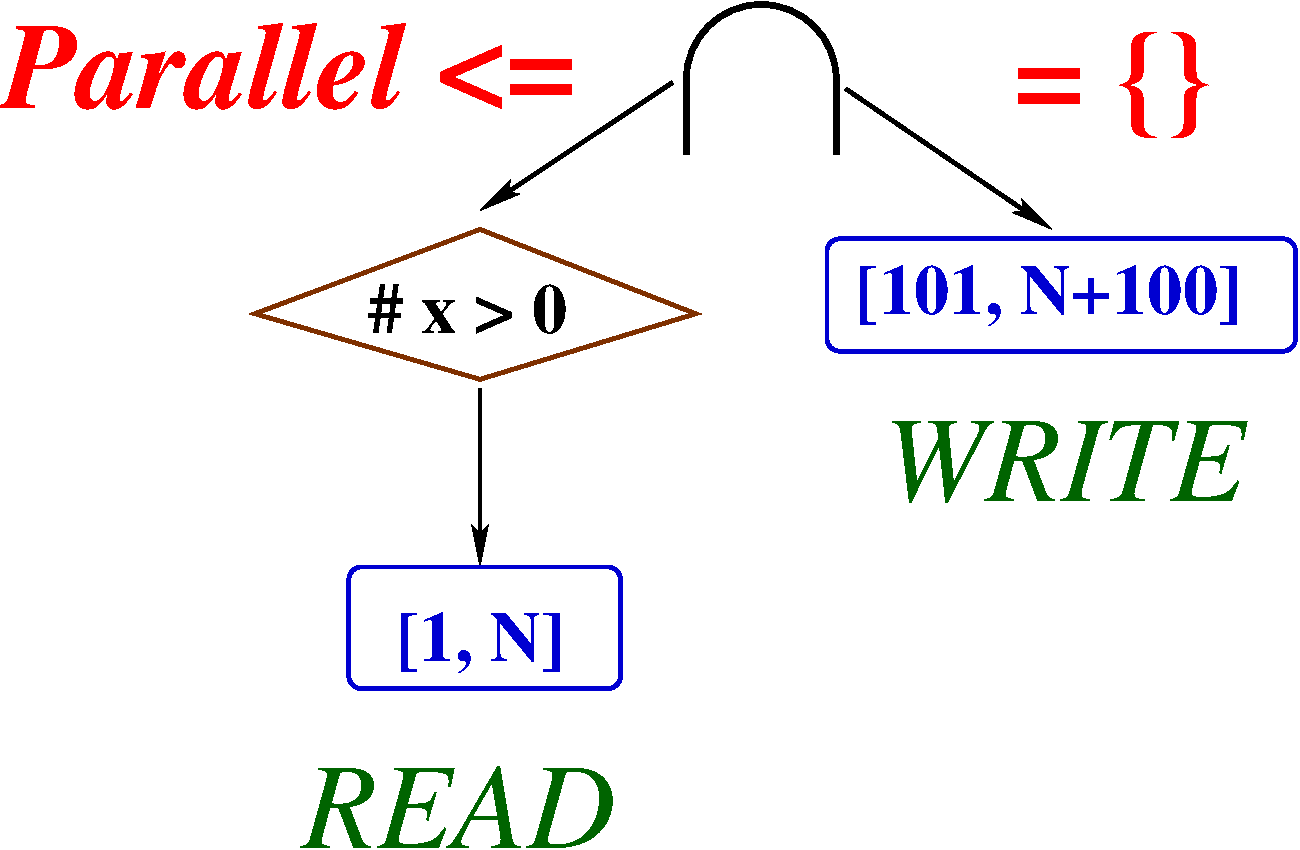
\includegraphics[height=15ex]{ParTeaserFigs/SimpleInd}
\end{center}
\end{columns}
\end{block}


        \begin{itemize}
            \item Techniques that analyze read-write pairs of accesses become
                    very conservative on larger loops with non-trivial control flow.\smallskip   
            \item {\em Alternative:} inter-procedural summarization + model loop independence 
                    via an equation on summaries of shape $S = \emptyset$\\\smallskip 
            \item Decrease overhead by extracting lightweight predicates that prove 
                    independence at runtime, e.g., {\tt x~$\leq$~0~~$\vee$~~N~<~100}.
        \end{itemize} 

\bigskip

\alert{Show Calculix from \textsc{Spec2006}}!

\end{frame}


\begin{frame}[fragile,t]
  \frametitle{Building RO, RW, WF Summaries Interprocedurally}

Summaries ({\sc ro}, {\sc rw}, {\sc wf}) are
\begin{itemize}
    \item constructed via a bottom-up parse of the {\sc call} and {\sc cd} graphs,
    \item structural data-flow equations dictate how to compose consecutive regions,
            aggregate/translate across loops/callsites, ...
\end{itemize}

\pause

\begin{block}{Simplified {\tt solvh\_do20} from {\tt dyfesm}} \vspace{-1ex}
\begin{columns} 
\column{0.45\textwidth}
\begin{colorcode}[fontsize=\scriptsize]
\emp{DO i = 1, N}
    CALL geteu (XE(IA(i)), NP, SYM)
    CALL matmul(XE(IA(i)), NS)
\emp{ENDDO}

SUBROUTINE matmul(XE, NS)
  INTEGER NS, XE(*)
  DO j = 1, NS
    ...   = XE(j) ...
    XE(j) = ...
  ENDDO 
END
\end{colorcode}
\column{0.45\textwidth} 
\begin{colorcode}[fontsize=\scriptsize]
SUBROUTINE geteu(XE, NP, SYM)
  INTEGER NP, SYM, XE(16, *)
  
  IF (SYM .NE. 1) THEN
    DO i = 1, NP
      DO j = 1, 16
        XE(j, i) = ...
      ENDDO 
    ENDDO
  ENDIF
END
\end{colorcode}
\end{columns}
\end{block}

\end{frame}


%%%%%%%%%%%%%%%%%%%%%%%%%%%%%%
%%%%% SUBROUTINE getue
%%%%%%%%%%%%%%%%%%%%%%%%%%%%%%

\begin{frame}[fragile,t]
  \frametitle{Summarizing Subroutine {\tt geteu}}

\begin{block}{WF summary for {\tt geteu}; RO$_{geteu}$ $=$ RW$_{geteu}$ $= \emptyset$ } \vspace{-1ex}
\begin{columns} 
\column{0.45\textwidth} 
\begin{colorcode}[fontsize=\scriptsize]
\mymath{S\myindx{geteu}}  SUBROUTINE geteu(XE, NP, SYM)
         INTEGER NP, SYM, XE(16, *)  
\mymath{S\myindx{IF}}       \emph{IF (SYM .NE. 1) THEN}
\mymath{S\myindx{Li}}         \emp{DO i = 1, NP}
\mymath{S\myindx{Lj}}           \emp{DO j = 1, 16}
\mymath{S\myindx{WF}}             \alert{XE(j, i)} = ...
             \emp{ENDDO} 
           \emp{ENDDO}
         \emph{ENDIF}
       END
\end{colorcode}
\column{0.45\textwidth}
\begin{colorcode}[fontsize=\scriptsize]








\alert{\mymath{WF\myindu{XE}\myindx{S\myindx{WF}} = \{16*i+j-1\}}}
\end{colorcode}
\end{columns}
\end{block}


\begin{itemize}
    \item Loop Aggregation uses (intuitively) interval arithmetic: \smallskip
    \item Loop $i$: $\{16*i + j - 1 \mbox{ }\mbox{ }|\mbox{ } j \in \{1..\mbox{ }16\}\} \rightarrow \emp{16*i + [0,15]}$ \smallskip
    \item Loop $j$: $\{16*i + [0,15] \mbox{ }|\mbox{ } i \in \{1..NP\}\} \rightarrow \emp{[0, 16*NP-1]}$  \smallskip
    \item Branches introduce predicated nodes, e.g., \emph{$WF^{XE}_{S_{if}} = WF^{XE}_{S_{geteu}}$} 
\end{itemize}
\end{frame}

%%%%%%%%%%%%%%%%%%%%%%%%%%%%%%%%%%%%%%%%%%%%%%%%%%%%

\begin{frame}[fragile,t]
  \frametitle{Summarizing Subroutine {\tt geteu}}

\begin{block}{WF summary for {\tt geteu}; RO$_{geteu}$ $=$ RW$_{geteu}$ $= \emptyset$ } \vspace{-1ex}
\begin{columns} 
\column{0.45\textwidth} 
\begin{colorcode}[fontsize=\scriptsize]
\mymath{S\myindx{geteu}}  SUBROUTINE geteu(XE, NP, SYM)
         INTEGER NP, SYM, XE(16, *)  
\mymath{S\myindx{IF}}       \emph{IF (SYM .NE. 1) THEN}
\mymath{S\myindx{Li}}         \emp{DO i = 1, NP}
\mymath{S\myindx{Lj}}           \emp{DO j = 1, 16}
\mymath{S\myindx{WF}}             \alert{XE(j, i)} = ...
             \emp{ENDDO} 
           \emp{ENDDO}
         \emph{ENDIF}
       END
\end{colorcode}
\column{0.45\textwidth}
\begin{colorcode}[fontsize=\scriptsize]

\emp{\mymath{WF\myindu{XE}\myindx{S\myindx{Lj}} = 16*i + [0,15]}}

\alert{\mymath{WF\myindu{XE}\myindx{S\myindx{WF}} = \{16*i+j-1\}}}
\end{colorcode}
\end{columns}
\end{block}


\begin{itemize}
    \item Loop Aggregation uses (intuitively) interval arithmetic: \smallskip
    \item Loop $i$: $\{16*i + j - 1 \mbox{ }\mbox{ }|\mbox{ } j \in \{1..\mbox{ }16\}\} \rightarrow \emp{16*i + [0,15]}$ \smallskip
    \item Loop $j$: $\{16*i + [0,15] \mbox{ }|\mbox{ } i \in \{1..NP\}\} \rightarrow \emp{[0, 16*NP-1]}$  \smallskip
    \item Branches introduce predicated nodes, e.g., \emph{$WF^{XE}_{S_{if}} = WF^{XE}_{S_{geteu}}$} 
\end{itemize}
\end{frame}


%%%%%%%%%%%%%%%%%%%%%%%%%%%%%%%%%%%%%%%%%%%%%%%%%%%%

\begin{frame}[fragile,t]
  \frametitle{Summarizing Subroutine {\tt geteu}}

\begin{block}{WF summary for {\tt geteu}; RO$_{geteu}$ $=$ RW$_{geteu}$ $= \emptyset$ } \vspace{-1ex}
\begin{columns} 
\column{0.45\textwidth} 
\begin{colorcode}[fontsize=\scriptsize]
\mymath{S\myindx{geteu}}  SUBROUTINE geteu(XE, NP, SYM)
         INTEGER NP, SYM, XE(16, *)  
\mymath{S\myindx{IF}}       \emph{IF (SYM .NE. 1) THEN}
\mymath{S\myindx{Li}}         \emp{DO i = 1, NP}
\mymath{S\myindx{Lj}}           \emp{DO j = 1, 16}
\mymath{S\myindx{WF}}             \alert{XE(j, i)} = ...
             \emp{ENDDO} 
           \emp{ENDDO}
         \emph{ENDIF}
       END
\end{colorcode}
\column{0.45\textwidth}
\begin{colorcode}[fontsize=\scriptsize]




\emp{\mymath{WF\myindu{XE}\myindx{S\myindx{Li}} = [0,16*NP-1]}}

\emp{\mymath{WF\myindu{XE}\myindx{S\myindx{Lj}} = 16*i + [0,15]}}

\alert{\mymath{WF\myindu{XE}\myindx{S\myindx{WF}} = \{16*i+j-1\}}}
\end{colorcode}
\end{columns}
\end{block}


\begin{itemize}
    \item Loop Aggregation uses (intuitively) interval arithmetic: \smallskip
    \item Loop $i$: $\{16*i + j - 1 \mbox{ }\mbox{ }|\mbox{ } j \in \{1..\mbox{ }16\}\} \rightarrow \emp{16*i + [0,15]}$ \smallskip
    \item Loop $j$: $\{16*i + [0,15] \mbox{ }|\mbox{ } i \in \{1..NP\}\} \rightarrow \emp{[0, 16*NP-1]}$  \smallskip
    \item Branches introduce predicated nodes, e.g., \emph{$WF^{XE}_{S_{if}} = WF^{XE}_{S_{geteu}}$} 
\end{itemize}
\end{frame}


%%%%%%%%%%%%%%%%%%%%%%%%%%%%%%%%%%%%%%%%%%%%%%%%%%%%

\begin{frame}[fragile,t]
  \frametitle{Summarizing Subroutine {\tt geteu}}

\begin{block}{WF summary for {\tt geteu}; RO$_{geteu}$ $=$ RW$_{geteu}$ $= \emptyset$ } \vspace{-1ex}
\begin{columns} 
\column{0.45\textwidth} 
\begin{colorcode}[fontsize=\scriptsize]
\mymath{S\myindx{geteu}}  SUBROUTINE geteu(XE, NP, SYM)
         INTEGER NP, SYM, XE(16, *)  
\mymath{S\myindx{IF}}       \emph{IF (SYM .NE. 1) THEN}
\mymath{S\myindx{Li}}         \emp{DO i = 1, NP}
\mymath{S\myindx{Lj}}           \emp{DO j = 1, 16}
\mymath{S\myindx{WF}}             \alert{XE(j, i)} = ...
             \emp{ENDDO} 
           \emp{ENDDO}
         \emph{ENDIF}
       END
\end{colorcode}
\column{0.45\textwidth}
\begin{colorcode}[fontsize=\scriptsize]
          \emph{\mymath{(SYM \neq 1)}}
\emph{\mymath{WF\myindu{XE}\myindx{S\myindx{IF}} =}       \mymath{\downarrow}}
          \emph{\mymath{[0,16*NP-1]}}

\emp{\mymath{WF\myindu{XE}\myindx{S\myindx{Li}} = [0,16*NP-1]}}

\emp{\mymath{WF\myindu{XE}\myindx{S\myindx{Lj}} = 16*i + [0,15]}}

\alert{\mymath{WF\myindu{XE}\myindx{S\myindx{WF}} = \{16*i+j-1\}}}
\end{colorcode}
\end{columns}
\end{block}


\begin{itemize}
    \item Loop Aggregation uses (intuitively) interval arithmetic: \smallskip
    \item Loop $i$: $\{16*i + j - 1 \mbox{ }\mbox{ }|\mbox{ } j \in \{1..\mbox{ }16\}\} \rightarrow \emp{16*i + [0,15]}$ \smallskip
    \item Loop $j$: $\{16*i + [0,15] \mbox{ }|\mbox{ } i \in \{1..NP\}\} \rightarrow \emp{[0, 16*NP-1]}$  \smallskip
    \item Branches introduce predicated nodes, e.g., \emph{$WF^{XE}_{S_{if}} = WF^{XE}_{S_{geteu}}$} 
\end{itemize}
\end{frame}


%%%%%%%%%%%%%%%%%%%%%%%%%%%%%%
%%%%% SUBROUTINE getue END
%%%%%%%%%%%%%%%%%%%%%%%%%%%%%%


%%%%% SUBROUTINE MATMULT

\begin{frame}[fragile,t]
  \frametitle{Summarizing Subroutine {\tt matmult}}

\begin{block}{RW summary for {\tt matmul}; RO$_{matmul}$ $=$ WF$_{matmul}$ $= \emptyset$ } \vspace{-1ex}
\begin{columns} 
\column{0.48\textwidth} 
\begin{colorcode}[fontsize=\scriptsize]
\mymath{S\myindx{matmul}}  SUBROUTINE matmul(XE, NS)
          INTEGER NS, XE(*)
\mymath{S\myindx{loop}}       \emph{DO j = 1, NS}
\mymath{S\myindx{RO}}          \alert{...   \hspace{0.5ex}= XE(j) ...}
\mymath{S\myindx{WF}}          \alert{XE(j) = ...}
          \emph{ENDDO}
        END
\end{colorcode}
\column{0.48\textwidth}
\begin{colorcode}[fontsize=\scriptsize]




\alert{\mymath{RO\myindu{XE}\myindx{S\myindx{RO}} = \{j-1\}}}
\alert{\mymath{WF\myindu{XE}\myindx{S\myindx{WF}} = \{j-1\}}}
\end{colorcode}
\end{columns}
\end{block}

\bigskip

\begin{itemize}
    \item Composing read-only $RO_{S_1}$ and write-first $WF_{S_2}$ regions:  \smallskip
    \item $RO = RO_{S_1} - WF_{S_2}$, $WF = WF_{S_2} - RO_{S_1}$, $RW = RO_{S_1} \cap WF_{S_2}$  \smallskip
    \item In our case $RO = \emptyset$, $WF = \emptyset$, \emp{$RW = \{j-1\}$}  \smallskip
    \item Over loop {\tt DO j}:  $RO_{loop} = \emptyset$, $WF_{loop} = \emptyset$, \emph{$RW_{loop} = [0, NS-1]$}  \smallskip
\end{itemize}
\end{frame}

%%%%%%%%%%%%%%%%%%%%%%%%%%%%%%%%%%%%%%%%%%%%%%%%%%%%

%%%%%%%%%%%%%%%%%%%%%%%%%%%%%%%%%%%%%%%%%%%%%%%%%%%%

\begin{frame}[fragile,t]
  \frametitle{Summarizing Subroutine {\tt matmult}}

\begin{block}{RW summary for {\tt matmul}; RO$_{matmul}$ $=$ WF$_{matmul}$ $= \emptyset$ } \vspace{-1ex}
\begin{columns} 
\column{0.48\textwidth} 
\begin{colorcode}[fontsize=\scriptsize]
\mymath{S\myindx{matmul}}  SUBROUTINE matmul(XE, NS)
          INTEGER NS, XE(*)
\mymath{S\myindx{loop}}       \emph{DO j = 1, NS}
\mymath{S\myindx{RO}}          \alert{...   \hspace{0.5ex}= XE(j) ...}
\mymath{S\myindx{WF}}          \alert{XE(j) = ...}
          \emph{ENDDO}
        END
\end{colorcode}
\column{0.48\textwidth}
\begin{colorcode}[fontsize=\scriptsize]


\emp{\mymath{S\myindx{RO} \diamond S\myindx{WF} = \{\emptyset, \emptyset, RW=\{j-1\}\}}}

\alert{\mymath{RO\myindu{XE}\myindx{S\myindx{RO}} = \{j-1\}}}
\alert{\mymath{WF\myindu{XE}\myindx{S\myindx{WF}} = \{j-1\}}}
\end{colorcode}
\end{columns}
\end{block}

\bigskip

\begin{itemize}
    \item Composing read-only $RO_{S_1}$ and write-first $WF_{S_2}$ regions:  \smallskip
    \item $RO = RO_{S_1} - WF_{S_2}$, $WF = WF_{S_2} - RO_{S_1}$, $RW = RO_{S_1} \cap WF_{S_2}$  \smallskip
    \item In our case $RO = \emptyset$, $WF = \emptyset$, \emp{$RW = \{j-1\}$}  \smallskip
    \item Over loop {\tt DO j}:  $RO_{loop} = \emptyset$, $WF_{loop} = \emptyset$, \emph{$RW_{loop} = [0, NS-1]$}  \smallskip
\end{itemize}
\end{frame}


\begin{frame}[fragile,t]
  \frametitle{Summarizing Subroutine {\tt matmult}}

\begin{block}{RW summary for {\tt matmul}; RO$_{matmul}$ $=$ WF$_{matmul}$ $= \emptyset$ } \vspace{-1ex}
\begin{columns} 
\column{0.48\textwidth} 
\begin{colorcode}[fontsize=\scriptsize]
\mymath{S\myindx{matmul}}  SUBROUTINE matmul(XE, NS)
          INTEGER NS, XE(*)
\mymath{S\myindx{loop}}       \emph{DO j = 1, NS}
\mymath{S\myindx{RO}}          \alert{...   \hspace{0.5ex}= XE(j) ...}
\mymath{S\myindx{WF}}          \alert{XE(j) = ...}
          \emph{ENDDO}
        END
\end{colorcode}
\column{0.48\textwidth}
\begin{colorcode}[fontsize=\scriptsize]
\emph{\mymath{RW\myindu{XE}\myindx{S\myindx{loop}} = [0,NS-1]}}

\emp{\mymath{S\myindx{RO} \diamond S\myindx{WF} = \{\emptyset, \emptyset, RW=\{j-1\}\}}}

\alert{\mymath{RO\myindu{XE}\myindx{S\myindx{RO}} = \{j-1\}}}
\alert{\mymath{WF\myindu{XE}\myindx{S\myindx{WF}} = \{j-1\}}}
\end{colorcode}
\end{columns}
\end{block}

\bigskip

\begin{itemize}
    \item Composing read-only $RO_{S_1}$ and write-first $WF_{S_2}$ regions:  \smallskip
    \item $RO = RO_{S_1} - WF_{S_2}$, $WF = WF_{S_2} - RO_{S_1}$, $RW = RO_{S_1} \cap WF_{S_2}$  \smallskip
    \item In our case $RO = \emptyset$, $WF = \emptyset$, \emp{$RW = \{j-1\}$}  \smallskip
    \item Over loop {\tt DO j}:  $RO_{loop} = \emptyset$, $WF_{loop} = \emptyset$, \emph{$RW_{loop} = [0, NS-1]$}  \smallskip
\end{itemize}
\end{frame}



%%%%% SUBROUTINE MATMULT

\begin{frame}[fragile,t]
  \frametitle{Summarizing Accesses for the Target Loop}

\begin{block}{RW summary for loop {\tt DO i}: RW$^i$ = ? } \vspace{-1ex}
\begin{columns} 
\column{0.48\textwidth} 
\begin{colorcode}[fontsize=\scriptsize]
        INTEGER NS, NP, IA(*), XE(*)
\mymath{S\myindx{loop}}    \emph{DO i = 1, N}
\mymath{S\myindx{WF}}      CALL geteu (XE(IA(i)),NP,SYM)
\mymath{S\myindx{RW}}      CALL matmul(XE(IA(i)),NS)
        \emph{ENDDO}

\emp{\mymath{S\myindx{WF} \diamond S\myindx{RW} = \{\emptyset, WF\myindu{i}=WF\myindx{geteu}, RW\myindu{i}\}}}
\end{colorcode}
\column{0.48\textwidth}
\begin{center}
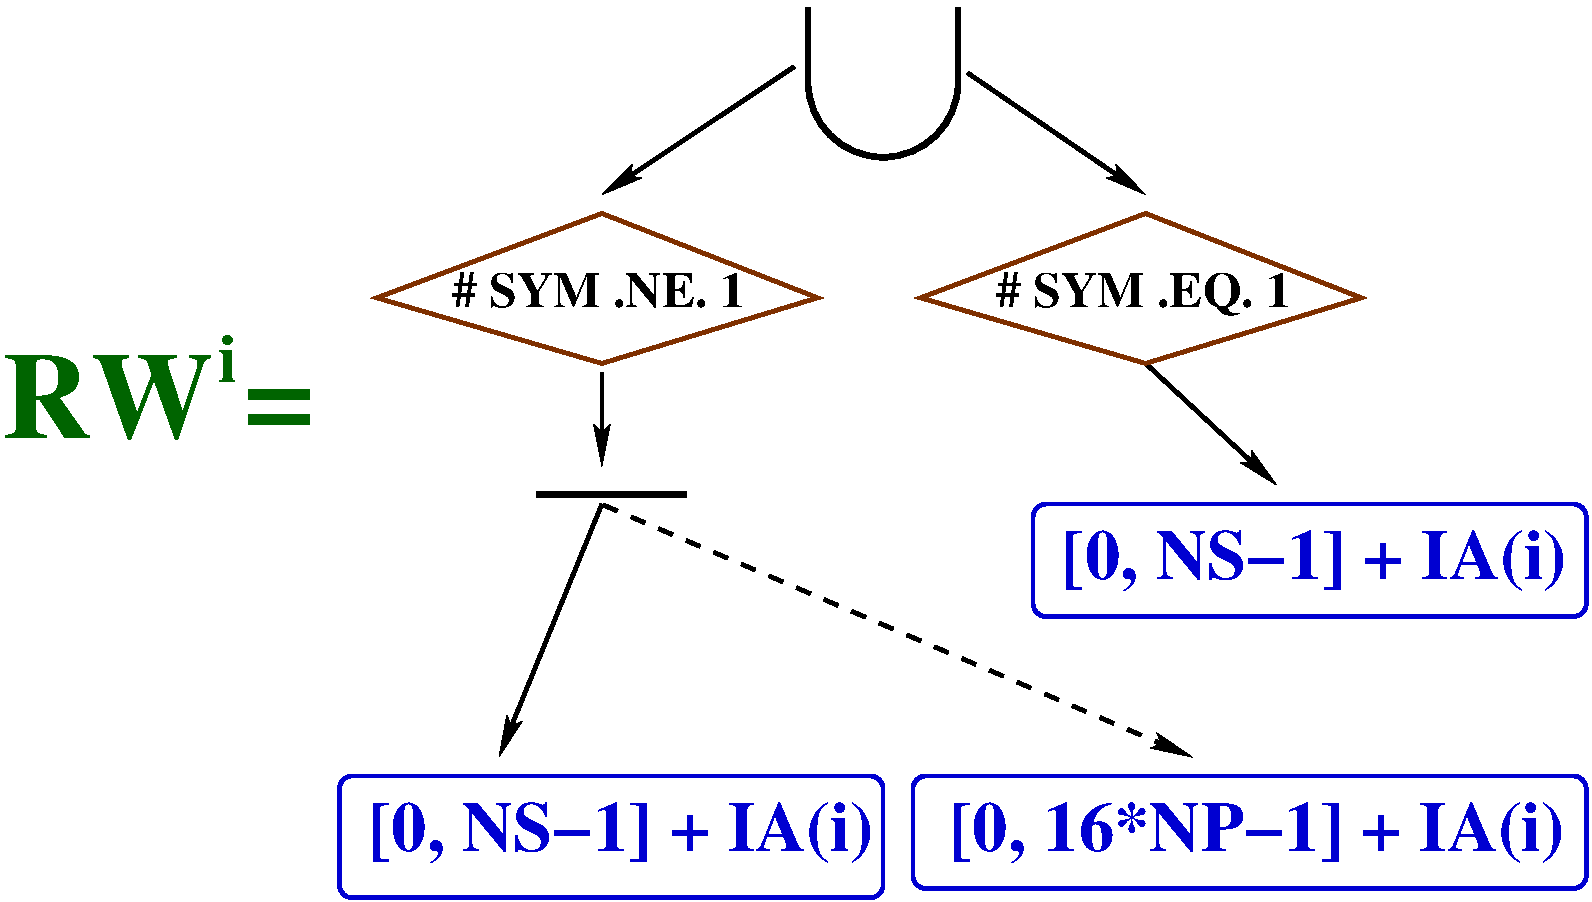
\includegraphics[height=15ex]{ParTeaserFigs/RW_IND_XE}
\end{center}
\end{columns}
\end{block}

\bigskip

In our case, a sufficient condition for {\tt XE} independence is: \bigskip \\ 
$\cup_{i=1}^{N}(RW_i \mbox{ }\cap\mbox{ } (\cup_{k=1}^{i-1}RW_k)) = \emptyset~~~\Leftrightarrow~~~RW_i = \emptyset~~~\Leftrightarrow$

\bigskip

$~~~~~~~~~~~~~~~~~\Leftrightarrow~~~$  
\emph{${\tt SYM}\neq 1\mbox{ }\wedge {\tt NS}\leq 16*{\tt NP}$} 
\end{frame}


\begin{frame}[fragile,t]
  \frametitle{Summary-Based Independence Equations}
\bigskip
Flow and Anti Independence Equation for loop of index \emph{i}:
\begin{equation} \label{FIEq} 
\begin{array}{l r}
S_{find} = \{(\cup_{i=1}^{N} WF_i) \mbox{ }\cap\mbox{ } (\cup_{i=1}^{N} RO_i)\} \mbox{ }\cup & \vspace{1ex} \\ \mbox{ }\mbox{ }\mbox{ }\mbox{ }\mbox{ }\mbox{ }\mbox{ }\mbox{ }\mbox{ }\mbox{ }
\{(\cup_{i=1}^{N} WF_i) \mbox{ }\cap\mbox{ } (\cup_{i=1}^{N} RW_i)\} \mbox{ }\cup & \vspace{1ex} \\ \mbox{ }\mbox{ }\mbox{ }\mbox{ }\mbox{ }\mbox{ }\mbox{ }\mbox{ }\mbox{ }\mbox{ }
\{(\cup_{i=1}^{N}RO_i) \mbox{ }\cap\mbox{ } (\cup_{i=1}^{N}RW_i)\} \mbox{ }\cup  & \vspace{1ex} \\ \mbox{ }\mbox{ }\mbox{ }\mbox{ }\mbox{ }\mbox{ }\mbox{ }\mbox{ }\mbox{ }\mbox{ }
\{ \cup_{i=1}^{N}(RW_i \mbox{ }\cap\mbox{ } (\cup_{k=1}^{i-1}RW_k))\} \mbox{ }\mbox{ }\mbox{ } = \emptyset
\end{array}
\end{equation}

\bigskip

Output Independence Equation for loop of index \emph{i}:
\begin{equation} \label{OIEq} 
\begin{array}{l r}
S_{oind} = \{ \cup_{i=1}^{N}(WF_i \mbox{ }\cap\mbox{ } (\cup_{k=1}^{i-1}WF_k))\} \mbox{ }\mbox{ }\mbox{ } = \emptyset
\end{array}
\end{equation}

\bigskip

Computing $S_{find}$ and $S_{oind}$ solves a more difficult problem than we need, 
i.e., computes the indexes involved in cross-iteration deps. \bigskip

\emp{{\em Loop Independence: when are $S_{find}$ and $S_{oind}$ are empty?}}

\end{frame}


\begin{frame}[fragile,t]
  \frametitle{Key Idea: Predicate-Centric Approach}

\smallskip

{\em Approach centered on extracting arbitrarily-shaped predicates.} 

\bigskip

\begin{block}{Key Idea} 
\begin{columns} 
\column{0.69\textwidth} \vspace{-2ex}
\begin{itemize}
    \item \emp{{\em Source of inaccuracy:}} summary representation not closed under composition w.r.t. set operations. \bigskip
    \item \emph{{\em Language}} representation for summaries ... precise but \emp{expensive} to compute at runtime \bigskip
    \item ``Let's \emph{{\em reason}} about it!'' $\emph{8*NP < NS + 6} \Rightarrow \emp{A - B} = \emptyset \Rightarrow S=\emptyset$!
\end{itemize}
\column{0.33\textwidth} 
\hspace{-2ex}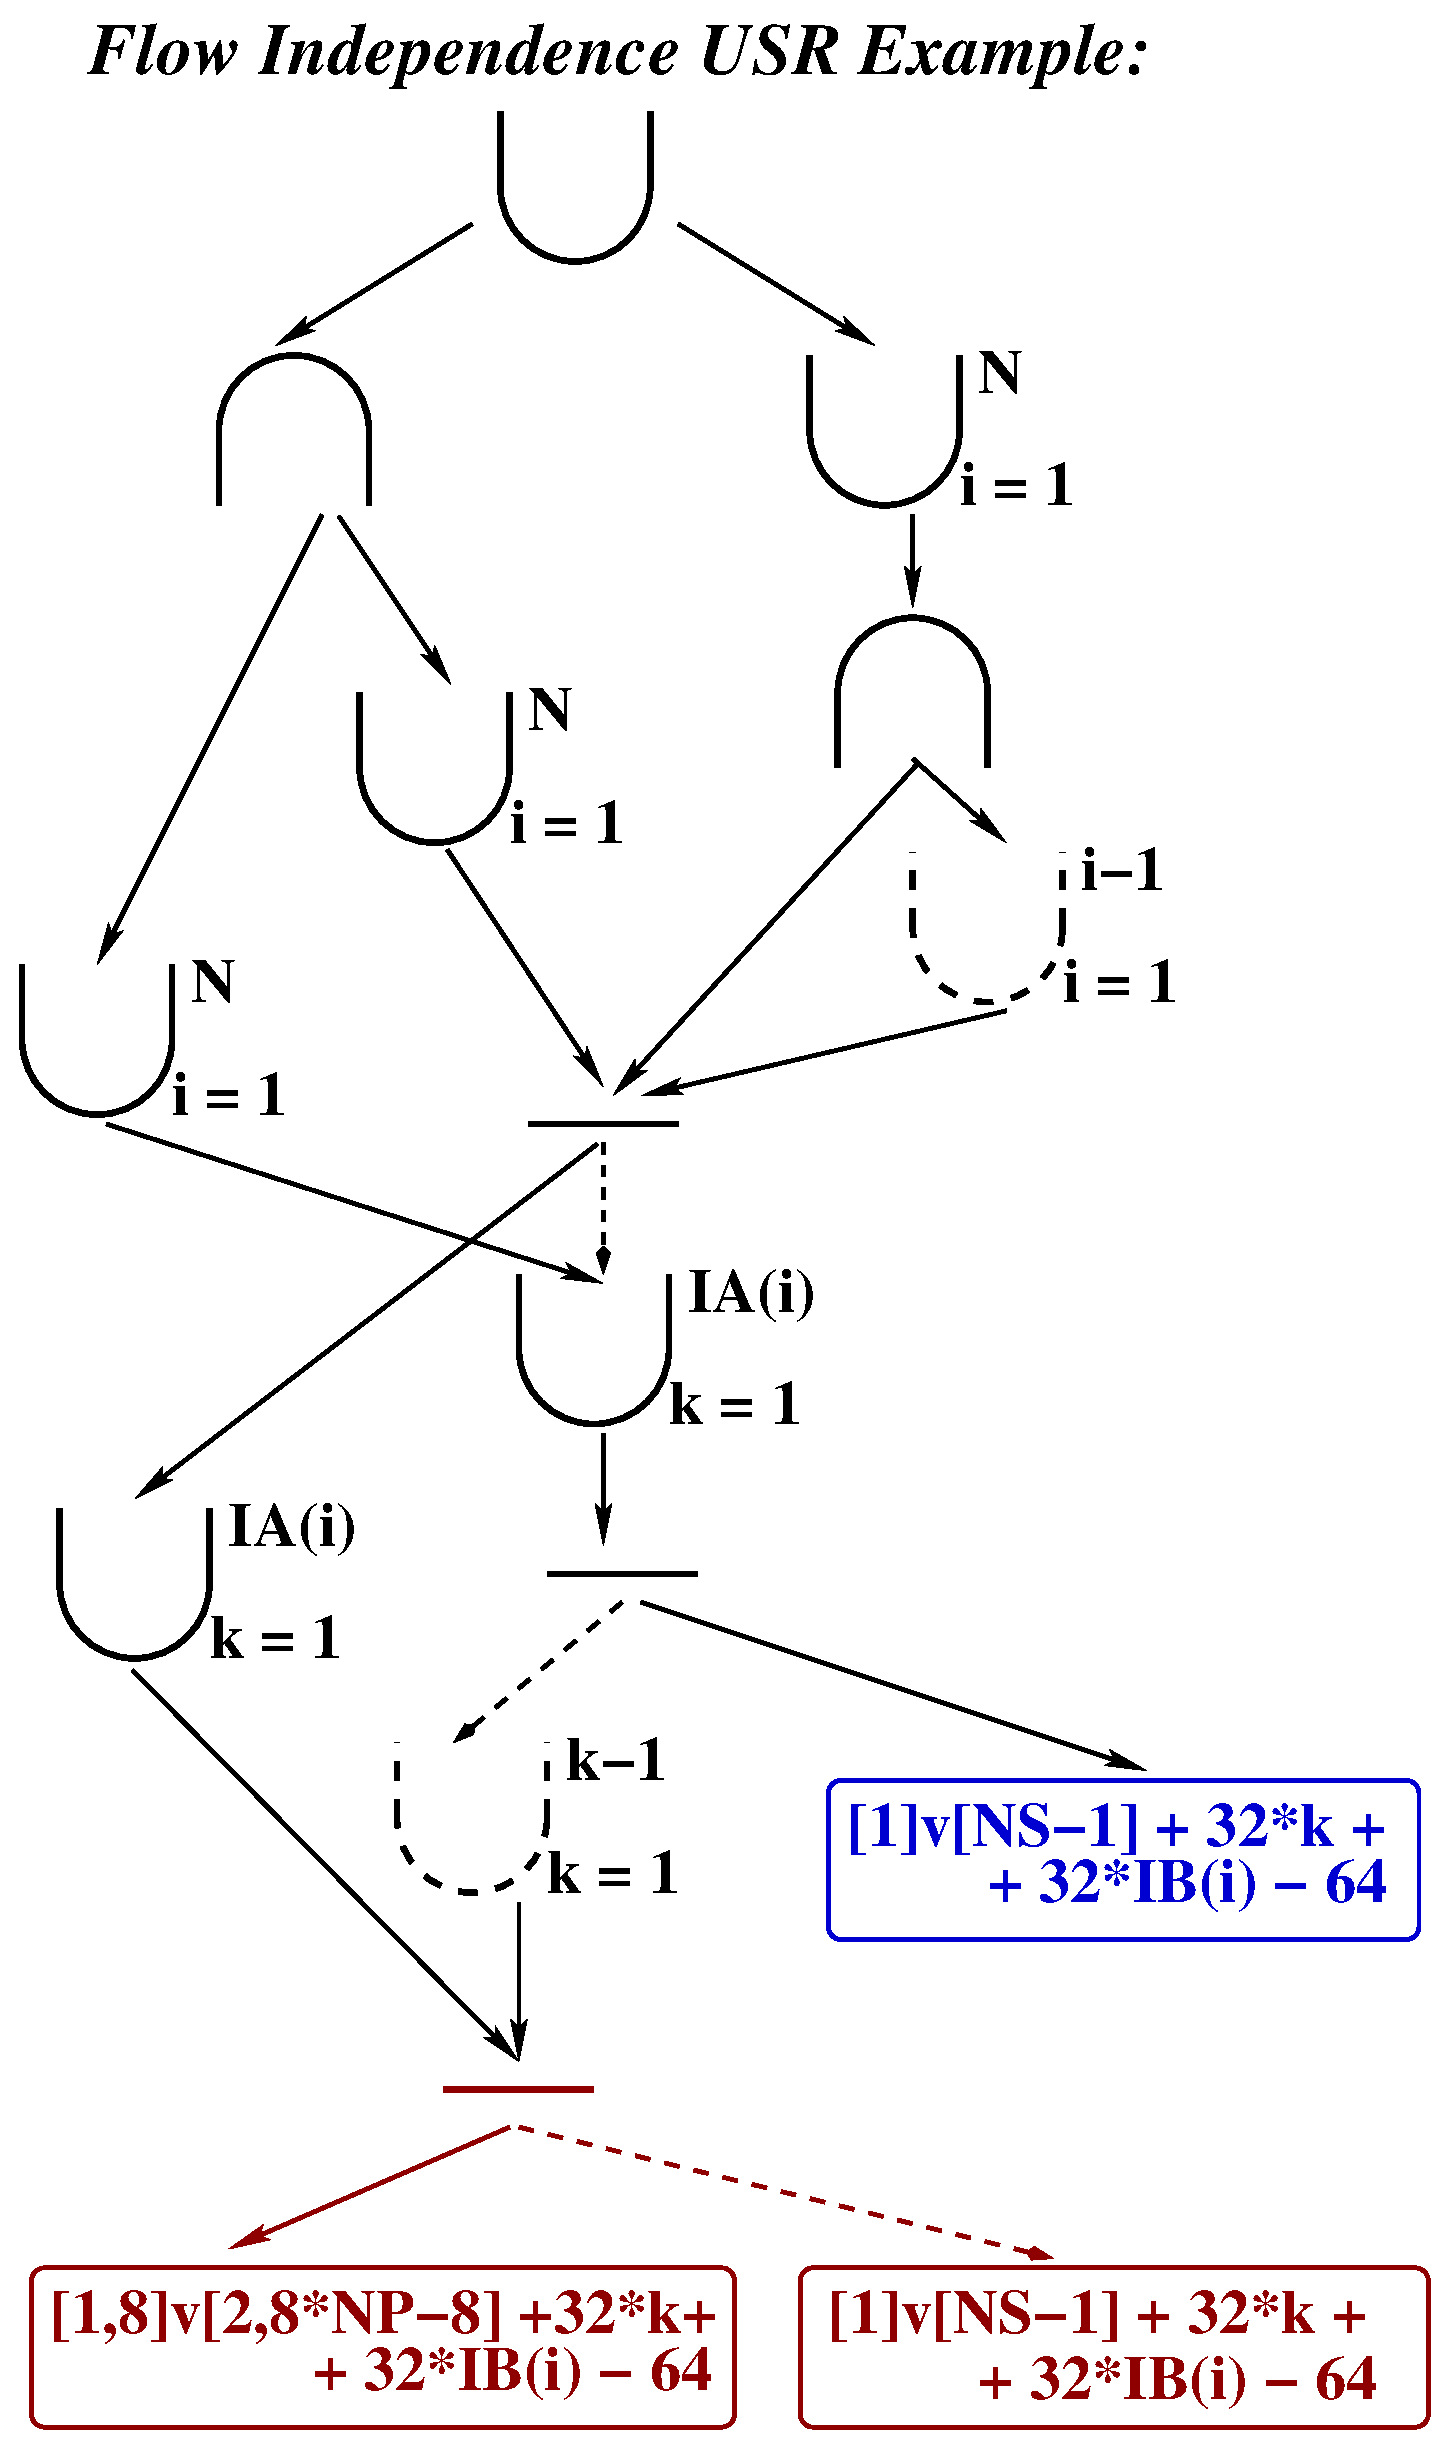
\includegraphics[height=30ex]{ParTeaserFigs/USR_HE_FIND_SOLVH}
\end{columns}
\end{block}

\alert{Show Calculix from \textsc{Spec2006}}!

\end{frame}

\end{document}

